\documentclass[english,notitlepage]{revtex4-1}  % defines the basic parameters of the document
%For preview: skriv i terminal: latexmk -pdf -pvc filnavn



% if you want a single-column, remove reprint

% allows special characters (including æøå)
\usepackage[utf8]{inputenc}
%\usepackage[english]{babel}

%% note that you may need to download some of these packages manually, it depends on your setup.
%% I recommend downloading TeXMaker, because it includes a large library of the most common packages.

\usepackage{physics,amssymb}  % mathematical symbols (physics imports amsmath)
\include{amsmath}
\usepackage{graphicx}         % include graphics such as plots
\usepackage{xcolor}           % set colors
\usepackage{hyperref}         % automagic cross-referencing (this is GODLIKE)
\usepackage{listings}         % display code
\usepackage{subfigure}        % imports a lot of cool and useful figure commands
\usepackage{float}
%\usepackage[section]{placeins}
\usepackage{algorithm}
\usepackage[noend]{algpseudocode}
\usepackage{subfigure}
\usepackage{tikz}
\usetikzlibrary{quantikz}
% defines the color of hyperref objects
% Blending two colors:  blue!80!black  =  80% blue and 20% black
\hypersetup{ % this is just my personal choice, feel free to change things
    colorlinks,
    linkcolor={red!50!black},
    citecolor={blue!50!black},
    urlcolor={blue!80!black}}

%% Defines the style of the programming listing
%% This is actually my personal template, go ahead and change stuff if you want



%% USEFUL LINKS:
%%
%%   UiO LaTeX guides:        https://www.mn.uio.no/ifi/tjenester/it/hjelp/latex/
%%   mathematics:             https://en.wikibooks.org/wiki/LaTeX/Mathematics

%%   PHYSICS !                https://mirror.hmc.edu/ctan/macros/latex/contrib/physics/physics.pdf

%%   the basics of Tikz:       https://en.wikibooks.org/wiki/LaTeX/PGF/Tikz
%%   all the colors!:          https://en.wikibooks.org/wiki/LaTeX/Colors
%%   how to draw tables:       https://en.wikibooks.org/wiki/LaTeX/Tables
%%   code listing styles:      https://en.wikibooks.org/wiki/LaTeX/Source_Code_Listings
%%   \includegraphics          https://en.wikibooks.org/wiki/LaTeX/Importing_Graphics
%%   learn more about figures  https://en.wikibooks.org/wiki/LaTeX/Floats,_Figures_and_Captions
%%   automagic bibliography:   https://en.wikibooks.org/wiki/LaTeX/Bibliography_Management  (this one is kinda difficult the first time)
%%   REVTeX Guide:             http://www.physics.csbsju.edu/370/papers/Journal_Style_Manuals/auguide4-1.pdf
%%
%%   (this document is of class "revtex4-1", the REVTeX Guide explains how the class works)


%% CREATING THE .pdf FILE USING LINUX IN THE TERMINAL
%%
%% [terminal]$ pdflatex template.tex
%%
%% Run the command twice, always.
%% If you want to use \footnote, you need to run these commands (IN THIS SPECIFIC ORDER)
%%
%% [terminal]$ pdflatex template.tex
%% [terminal]$ bibtex template
%% [terminal]$ pdflatex template.tex
%% [terminal]$ pdflatex template.tex
%%
%% Don't ask me why, I don't know.

\begin{document}

\title{Title of the document}      % self-explanatory
\author{Jon Aleksander Prøitz and Marius Torsvoll}          % self-explanatory
\date{\today}                             % self-explanatory
\noaffiliation                            % ignore this, but keep it.

\begin{abstract}
    Url to GitHub reposotory: \url{https://github.com/Jonaproitz/H21_Project_2_3150}
\end{abstract}
\maketitle 
    

\section*{Problem 1.}
    Given
    \begin{equation}
            \gamma \frac{d^2 u(x)}{d x^2}
        =   -Fu(x)
        \label{eq4}
    \end{equation}
    with the definition $\hat{x} = x/L$, such that
    \begin{equation*}
            \frac{d\hat{x}}{d x}
        =   \frac{1}{L}
        \implies 
            dx
        =   L d\hat{x}
    \end{equation*}
    Equation \ref{eq4} can be written
    \begin{equation*}
            \gamma \frac{d^2 u(\hat{x})}{L^2 d\hat{x}^2}
        =   -Fu(\hat{x})
        \implies
            \frac{d^2 u(\hat{x})}{d \hat{x}^2}
        =   -\frac{FL^2}{\gamma}u(\hat{x})
        =   -\lambda u(\hat{x})
    \end{equation*}
    with $\lambda = FL^2/\gamma$.$\hfill\blacksquare$


\section*{Problem 2.}
    For an arbitrary composite matrix $A = BC$ the transpose of $A^T = (BC)^T = C^TB^T$.
    Hence for $\vec{w}_i = U\vec{v}_i$
    \begin{equation*}
            \vec{w}^T_i\vec{w}_j
        =   \vec{v}^T_iU^TU\vec{v}_j
        =   \vec{v}^T_i\vec{v}_i
        =   \delta_{i,j}
    \end{equation*}
    as $U^TU = U^{-1}U = I$


\section*{Problem 3.}
The calculated values is to be found below. From table 13 to 26 the eigenvalue of the numerical and
analytical solution can be found. The expected analytical and the numerical value is are very close 
to each other. 
    \begin{table}[!ht]
        \begin{minipage}{0.4\textwidth}
            \centering
                \caption{Eigenvalue number 1.}
                \begin{tabular}{c@{\hspace{1cm}} c@{\hspace{1cm}} c}
                    \hline
                    arma::eig\_sym & Analytic & Difference \\
                    \hline
                    -74.2949 & -74.2949 & 0\\
                    \hline
                \end{tabular}
                \label{P3 eigenval 1}

            \vspace{.5cm}

            \centering
            \caption{Eigenvector number 1.}
            \begin{tabular}{c@{\hspace{1cm}} c@{\hspace{1cm}} c}
                \hline
                arma::eig\_sym & Analytic & Difference \\
                \hline
                -0.231921 & -0.231921 & 1.11022e-16\\
                -0.417907 & -0.417907 &1.11022e-16\\
                -0.521121 & -0.521121 & 3.33067e-16\\
                -0.521121 & -0.521121 & 3.33067e-16\\
                -0.417907 & -0.417907 & 3.33067e-16\\
                -0.231921 & -0.231921 & 3.33067e-16\\
                \hline
            \end{tabular}
            \label{P3 eigenvec 1}
            
        \end{minipage}
        \hspace{1.5cm}
        \begin{minipage}{0.4\textwidth}
            \centering
                \caption{Eigenvalue number 2.}
                \begin{tabular}{c@{\hspace{1cm}} c@{\hspace{1cm}} c}
                    \hline
                    arma::eig\_sym & Analytic & Difference \\
                    \hline
                    -47.102 & -47.102 & 2.13163e-14\\
                    \hline
                \end{tabular}
                \label{P3 eigenval 2}

            \vspace{.5cm}

            \centering
            \caption{Eigenvector number 2.}
            \begin{tabular}{c@{\hspace{1cm}} c@{\hspace{1cm}} c}
                \hline
                arma::eig\_sym & Analytic & Difference \\
                \hline
                -0.417907 & -0.417907 & 1.66533e-16\\
                -0.521121 & -0.521121 & 1.11022e-16\\
                -0.231921 & -0.231921 & 8.32667e-17\\
                 0.231921 &  0.231921 & 1.94289e-16\\
                 0.521121 &  0.521121 & 2.22045e-16\\
                 0.417907 &  0.417907 & 2.77556e-16\\
                \hline
            \end{tabular}
            \label{P3 eigenvec 2}
            
        \end{minipage}
    \end{table}

      
    \begin{table}[!ht]
        \begin{minipage}{0.4\textwidth}
            \centering
                \caption{Eigenvalue number 3.}
                \begin{tabular}{c@{\hspace{1cm}} c@{\hspace{1cm}} c}
                    \hline
                    arma::eig\_sym & Analytic & Difference \\
                    \hline
                    -7.80705 & -7.80705 & 5.32907e-15\\
                    \hline
                \end{tabular}
                \label{P3 eigenval 3}
            
            \vspace{.5cm}

            \centering
            \caption{Eigenvector number 3.}
            \begin{tabular}{c@{\hspace{1cm}} c@{\hspace{1cm}} c}
                \hline
                arma::eig\_sym & Analytic & Difference \\
                \hline
                -0.521121 & -0.521121 & 4.44089e-16\\
                -0.231921 & -0.231921 & 1.66533e-16\\
                 0.417907 &  0.417907 & 0\\
                 0.417907 &  0.417907 & 2.77556e-16\\
                -0.231921 & -0.231921 & 6.66134e-16\\
                -0.521121 & -0.521121 & 2.22045e-16\\
                \hline
            \end{tabular}
            \label{P3 eigenvec 3}
            \vspace{.5cm}
            
        \end{minipage}
        \hspace{1.5cm}
        \begin{minipage}{0.4\textwidth}
            \centering
                \caption{Eigenvalue number 4.}
                \begin{tabular}{c@{\hspace{1cm}} c@{\hspace{1cm}} c}
                    \hline
                    arma::eig\_sym & Analytic & Difference \\
                    \hline
                    35.8071 & 35.8071 & 2.13163e-14\\
                    \hline
                \end{tabular}
                \label{P3 eigenval 4}

            \vspace{.5cm}

            \centering
            \caption{Eigenvector number 4.}
            \begin{tabular}{c@{\hspace{1cm}} c@{\hspace{1cm}} c}
                \hline
                arma::eig\_sym & Analytic & Difference \\
                \hline
                -0.521121 & -0.521121 & 2.22045e-16\\
                 0.231921 &  0.231921 & 2.77556e-16\\
                 0.417907 &  0.417907 & 1.66533e-16\\
                -0.417907 & -0.417907 & 1.66533e-16\\
                -0.231921 & -0.231921 & 1.66533e-16\\
                 0.521121 &  0.521121 & 2.22045e-16\\
                \hline
            \end{tabular}
            \label{P3 eigenvec 4}
            \vspace{.5cm}
            
        \end{minipage}
    \end{table}


    \begin{table}[!ht]
        \begin{minipage}{0.4\textwidth}
            \centering
            \caption{Eigenvalue number 5.}
            \begin{tabular}{c@{\hspace{1cm}} c@{\hspace{1cm}} c}
                \hline
                arma::eig\_sym & Analytic & Difference \\
                \hline
                75.102 & 75.102 & 0\\
                \hline
            \end{tabular}
            \label{P3 eigenval 5}

        \vspace{.5cm}

        \centering
        \caption{Eigenvector number 5.}
        \begin{tabular}{c@{\hspace{1cm}} c@{\hspace{1cm}} c}
            \hline
            arma::eig\_sym & Analytic & Difference \\
            \hline
            -0.417907 & -0.417907 & 1.11022e-16\\
             0.521121 &  0.521121 & 6.66134e-16\\
            -0.231921 & -0.231921 & 3.05311e-16\\
            -0.231921 & -0.231921 & 1.38778e-16\\
             0.521121 &  0.521121 & 2.22045e-16\\
            -0.417907 & -0.417907 & 3.88578e-16\\
            \hline
        \end{tabular}
        \label{P3 eigenvec 5}
        \vspace{.5cm}
            
        \end{minipage}
        \hspace{1.5cm}
        \begin{minipage}{0.4\textwidth}
            \centering
            \caption{Eigenvalue number 6.}
            \begin{tabular}{c@{\hspace{1cm}} c@{\hspace{1cm}} c}
                \hline
                arma::eig\_sym & Analytic & Difference \\
                \hline
                102.295 & 102.295 & 0\\
                \hline
            \end{tabular}
            \label{P3 eigenval 6}

        \vspace{.5cm}

            \centering
            \caption{Eigenvector number 6.}
            \begin{tabular}{c@{\hspace{1cm}} c@{\hspace{1cm}} c}
                \hline
                arma::eig\_sym & Analytic & Difference \\
                \hline
                -0.231921 & -0.231921 & 0\\
                0.417907 &  0.417907 & 1.11022e-16\\
                -0.521121 & -0.521121 & 3.33067e-16\\
                0.521121 &  0.521121 & 1.11022e-16\\
                -0.417907 & -0.417907 & 3.33067e-16\\
                0.231921 &  0.231921 & 1.94289e-16\\
                \hline
            \end{tabular}
            \label{P3 eigenvec 6}
            \vspace{.5cm}
            
        \end{minipage}
    \end{table}\newpage


\section*{Problem 4.}
    The script found at the url at the top of the page returns 0.7. 
    Which is to be expected as the returned value is supposed to be the highest absolute
    value not on the diagonal of the matrix.  

\section*{Problem 5.}
The calculated values is to be found below. From table 13 to 26 the eigenvalue of the numerical and
analytical solution can be found. The expected analytical and the numerical value is are very close 
to each other. These values are somewhat less accurate than in problem 3. 

    \begin{table}[!ht]
        \begin{minipage}{0.4\textwidth}
            \centering
                \caption{Eigenvalue number 1.}
                \begin{tabular}{c@{\hspace{1cm}} c@{\hspace{1cm}} c}
                    \hline
                    arma::eig\_sym & Analytic & Difference \\
                    \hline
                    -74.2949 & -74.2949 & 2.84217e-14\\
                    \hline
                \end{tabular}
                \label{P5 eigenval 1}

            \vspace{.5cm}

            \centering
            \caption{Eigenvector number 1.}
            \begin{tabular}{c@{\hspace{1cm}} c@{\hspace{1cm}} c}
                \hline
                arma::eig\_sym & Analytic & Difference \\
                \hline
                -0.231921 & -0.231921 & 4.72591e-11\\
                -0.417907 & -0.417907 & 4.07815e-11\\
                -0.521121 & -0.521121 & 2.62265e-11\\
                -0.521121 & -0.521121 & 1.81499e-11\\
                -0.417907 & -0.417907 & 5.89315e-11\\
                -0.231921 & -0.231921 & 3.27045e-11\\
                \hline
            \end{tabular}
            \label{P5 eigenvec 1}
            
        \end{minipage}
        \hspace{1.5cm}
        \begin{minipage}{0.4\textwidth}
            \centering
                \caption{Eigenvalue number 2.}
                \begin{tabular}{c@{\hspace{1cm}} c@{\hspace{1cm}} c}
                    \hline
                    arma::eig\_sym & Analytic & Difference \\
                    \hline
                    -47.102 & -47.102 & 7.10543e-14\\
                    \hline
                \end{tabular}
                \label{P5 eigenval 2}

            \vspace{.5cm}

            \centering
            \caption{Eigenvector number 2.}
            \begin{tabular}{c@{\hspace{1cm}} c@{\hspace{1cm}} c}
                \hline
                arma::eig\_sym & Analytic & Difference \\
                \hline
                -0.417907 & -0.417907 &  2.61546e-11\\
                -0.521121 & -0.521121 &  3.27957e-11\\
                -0.231921 & -0.231921 &  5.88911e-11\\
                0.231921 & 0.231921 &  4.07412e-11\\
                0.521121 & 0.521121 &  4.73492e-11\\
                0.417907 & 0.417907 &  1.80767e-11\\
                \hline
            \end{tabular}
            \label{P5 eigenvec 2}
            
        \end{minipage}
    \end{table}

    
    \begin{table}[!ht]
        \begin{minipage}{0.4\textwidth}
            \centering
                \caption{Eigenvalue number 3.}
                \begin{tabular}{c@{\hspace{1cm}} c@{\hspace{1cm}} c}
                    \hline
                    arma::eig\_sym & Analytic & Difference \\
                    \hline
                    -7.80705 & -7.80705 & 6.21725e-15\\
                    \hline
                \end{tabular}
                \label{P5 eigenval 3}
            
            \vspace{.5cm}

            \centering
            \caption{Eigenvector number 3.}
            \begin{tabular}{c@{\hspace{1cm}} c@{\hspace{1cm}} c}
                \hline
                arma::eig\_sym & Analytic & Difference \\
                \hline
                -0.521121 & -0.521121 &  9.02611e-14\\
                -0.231921 & -0.231921 &  4.03566e-14\\
                0.417907 & 0.417907 &  7.25531e-14\\
                0.417907 & 0.417907 &  7.27196e-14\\
                -0.231921 & -0.231921 &  4.06897e-14\\
                -0.521121 & -0.521121 &  9.09273e-14\\
                \hline
            \end{tabular}
            \label{P5 eigenvec 3}
            \vspace{.5cm}
            
        \end{minipage}
        \hspace{1.5cm}
        \begin{minipage}{0.4\textwidth}
            \centering
                \caption{Eigenvalue number 4.}
                \begin{tabular}{c@{\hspace{1cm}} c@{\hspace{1cm}} c}
                    \hline
                    arma::eig\_sym & Analytic & Difference \\
                    \hline
                    35.8071 & 35.8071 & 1.42109e-14\\
                    \hline
                \end{tabular}
                \label{P5 eigenval 4}

            \vspace{.5cm}

            \centering
            \caption{Eigenvector number 4.}
            \begin{tabular}{c@{\hspace{1cm}} c@{\hspace{1cm}} c}
                \hline
                arma::eig\_sym & Analytic & Difference \\
                \hline
                -0.521121 & -0.521121 &  9.09273e-14\\
                0.231921 & 0.231921 &  4.03844e-14\\
                0.417907 & 0.417907 &  7.28306e-14\\
                -0.417907 & -0.417907 &  7.27196e-14\\
                -0.231921 & -0.231921 &  4.06897e-14\\
                0.521121 & 0.521121 &  9.03722e-14\\
                \hline
            \end{tabular}
            \label{P5 eigenvec 4}
            \vspace{.5cm}
            
        \end{minipage}
    \end{table}


    \begin{table}[!ht]
        \begin{minipage}{0.4\textwidth}
            \centering
            \caption{Eigenvalue number 5.}
            \begin{tabular}{c@{\hspace{1cm}} c@{\hspace{1cm}} c}
                \hline
                arma::eig\_sym & Analytic & Difference \\
                \hline
                75.102 & 75.102 & 4.26326e-14\\
                \hline
            \end{tabular}
            \label{P5 eigenval 5}

        \vspace{.5cm}

        \centering
        \caption{Eigenvector number 5.}
        \begin{tabular}{c@{\hspace{1cm}} c@{\hspace{1cm}} c}
            \hline
            arma::eig\_sym & Analytic & Difference \\
            \hline
            -0.417907 & -0.417907 &  2.63001e-11\\
            0.521121 & 0.521121 &  3.26146e-11\\
            -0.231921 & -0.231921 &  5.89711e-11\\
            -0.231921 & -0.231921 &  4.08214e-11\\
            0.521121 & 0.521121 &  4.71678e-11\\
            -0.417907 & -0.417907 &  1.82227e-11\\
            \hline
        \end{tabular}
        \label{P5 eigenvec 5}
        \vspace{.5cm}
            
        \end{minipage}
        \hspace{1.5cm}
        \begin{minipage}{0.4\textwidth}
            \centering
            \caption{Eigenvalue number 6.}
            \begin{tabular}{c@{\hspace{1cm}} c@{\hspace{1cm}} c}
                \hline
                arma::eig\_sym & Analytic & Difference \\
                \hline
                102.295 & 102.295 & 7.10543e-14\\
                \hline
            \end{tabular}
            \label{P5 eigenval 6}

        \vspace{.5cm}

            \centering
            \caption{Eigenvector number 6.}
            \begin{tabular}{c@{\hspace{1cm}} c@{\hspace{1cm}} c}
                \hline
                arma::eig\_sym & Analytic & Difference \\
                \hline
                -0.231921 & -0.231921 &  4.72589e-11\\
                0.417907 & 0.417907 &  4.07812e-11\\
                -0.521121 & -0.521121 &  2.62262e-11\\
                0.521121 & 0.521121 &  1.815e-11\\
                -0.417907 & -0.417907 &  5.89307e-11\\
                0.231921 & 0.231921 &  3.27042e-11\\
                \hline
            \end{tabular}
            \label{P5 eigenvec 6}
            \vspace{.5cm}
            
        \end{minipage}
    \end{table}\newpage


\section*{Problem 6.}
The change of the number of iterations behaves like the quadratic function. This was expected
    \begin{figure}
        \centering
        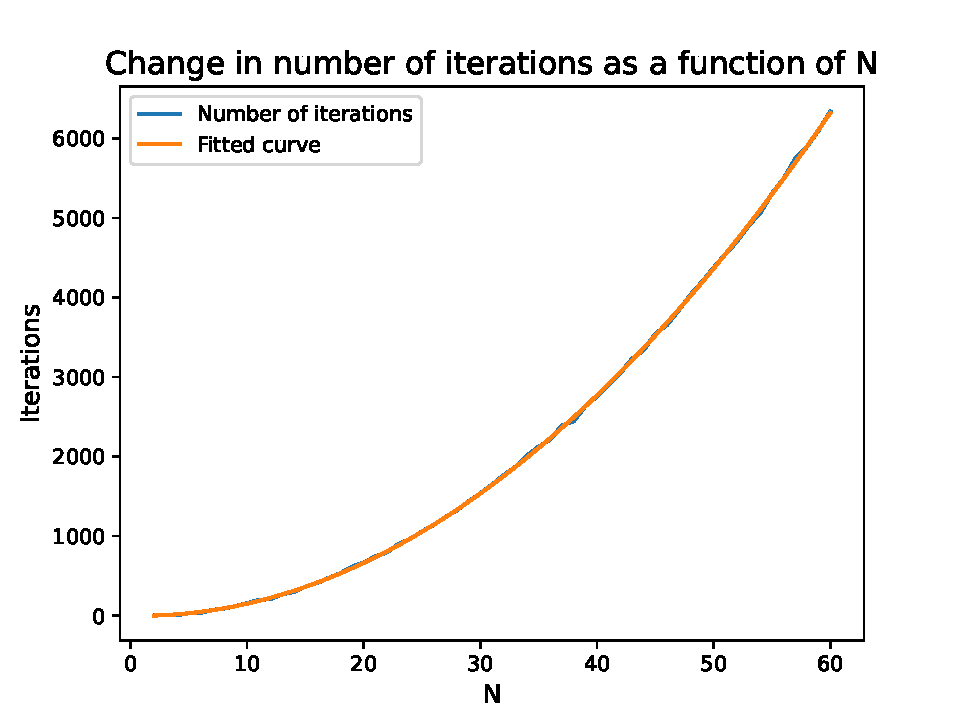
\includegraphics[scale=0.85]{iterations.pdf}
        \caption{}
        \label{iterations}
    \end{figure}
\section*{B}
We expect nothing to change as the algorithm will adjust all values in the matrix. This may be verified
by running the algorithm for a dense matrix. 

\section*{Problem 7.}
The Eigenvectors plotted for n = 10 and for n = 100 plotted with the analytical solution. As 
expected the N = 100 solution is alot smoother and a more accurate representation of the analytical
solution. 
\begin{figure}
    \centering
    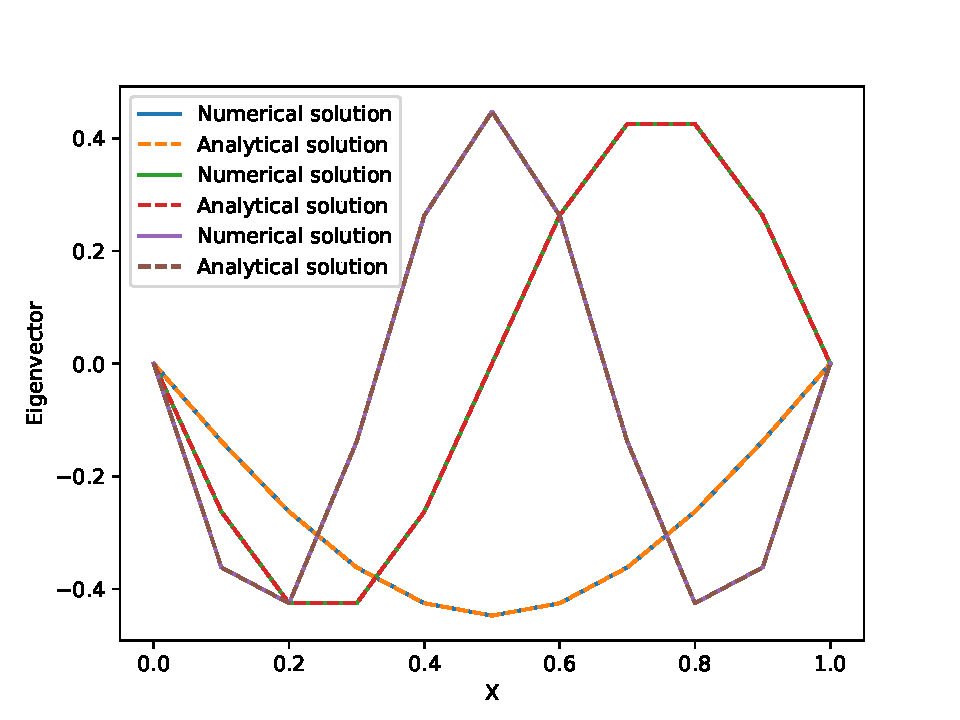
\includegraphics[scale=0.85]{Eigenvec10.pdf}
    \caption{Plotted for N = 10}
    \label{Eigenvector}
\end{figure}

\begin{figure}
    \centering
    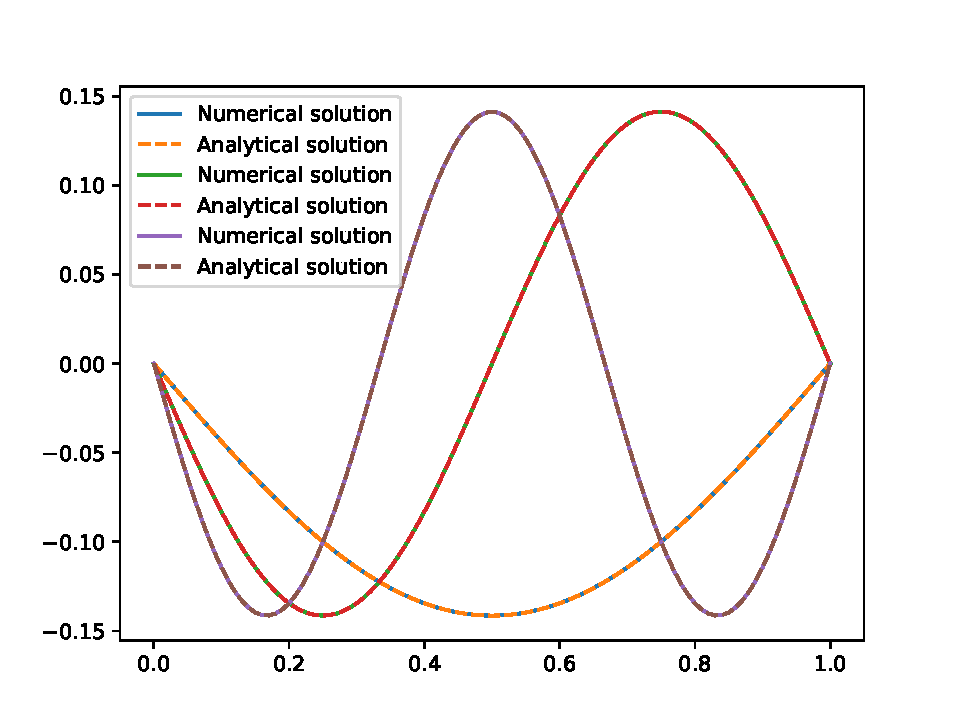
\includegraphics[scale=0.85]{Eigenvec100.pdf}
    \caption{Plotted for N = 100. }
    \label{Eigenvector100}
\end{figure}
\end{document}
